\section{Methods}

\subsection{MABE}

In this work we use the Modular Agent-Based Evolver\cite{bohm_mabe_2017} (MABE) framework to build and run our experiments. MABE allows for the quick construction of agent-based evolution simulations by allowing the scientist to reuse aspects of the system that have already been built by other members of the MABE community. In our work, we use the modules for Markov Brains, Circular Haploid Genomes, simple mutation-only reproduction via roulette selection, and population data archiving. Our contribution is therefore minimized to simply creating the world module, the module that defines the environment the agent will be evaluated in.

\subsection {Stigmergy World}

The world module is responsible for defining three key aspects of the simulation: The environment, how the agent senses the environment, and how the agent can change the environment.

In this work, the environment is an $n\times m$ grid surrounded by a wall and filled with smaller wall segments that create obstructions for the agent to navigate around. In addition, the environment contains one home location, where the agent will begin each simulation, and a food location. The environment is constructed by first generating a maze and then removing walls until the desired density of obstacles is reached (Figure \ref{fig:world_explanatory}). This method was chosen to ensure that home and food locations are always reachable by some path through the obstacles.

\begin{figure}
\begin{center}
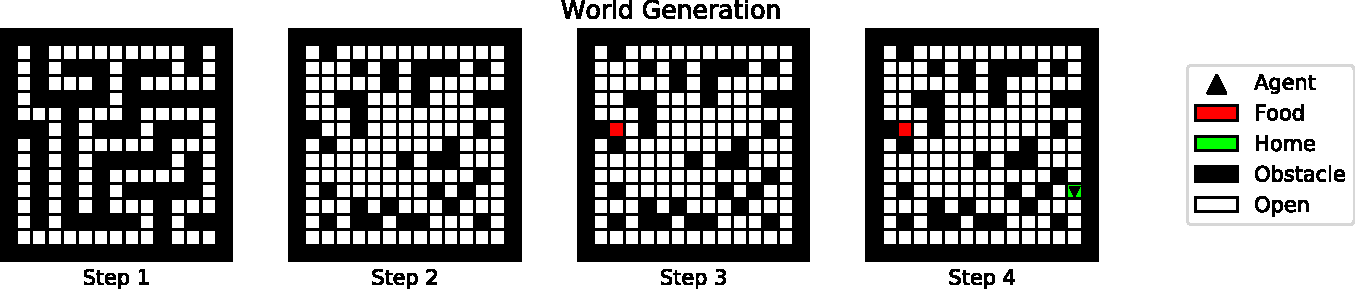
\includegraphics[width=\textwidth]{img/world_explanatory}
\caption{
Caption TODO
}
\label{fig:world_explanatory}
\end{center}
\end{figure}


The maze layout, wall removal, home location, and initial food location are all generated randomly during environment construction. A new environment is created before every agent evaluation. Furthermore, the location of food may change during an agent's lifetime according to the rules for food use. When the food must move, it is randomly relocated.
The agent is equipped with a total of $43+k$ bits of sensor data (Figure \ref{fig:sense_explanatory}). The agent has a vision cone that covers 8 cells with the capability of distinguishing 4 environmental states at each location (32 bits), a $3\times 3$ stigmergy proximity sensor centered on the agent's location (9 bits), an internal compass that provides a two-bit representation of the four cardinal directions, and a stigmergy read sensor that senses the $k$ bit stigmergy signal. In this work we have set $k$ to be $1$, disallowing the agent access to multiple, distinguishable, stigmergy signals. The agent receives input from each of its sensors at every world update.

\begin{figure}
\begin{center}
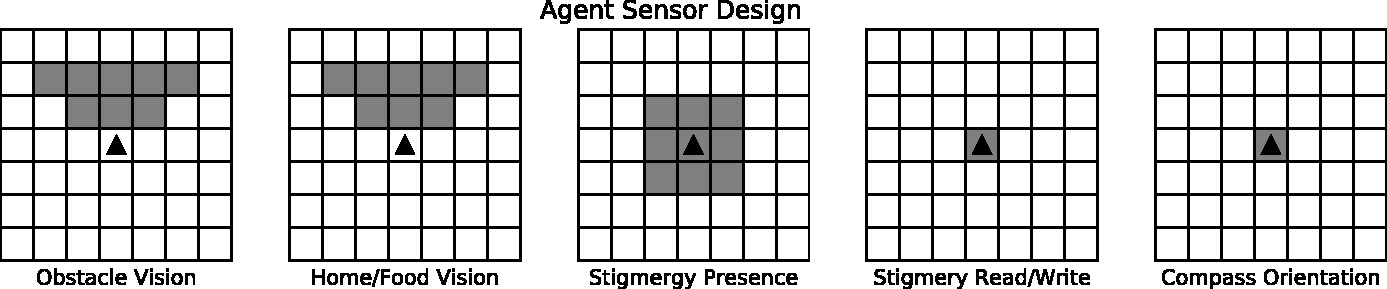
\includegraphics[width=\textwidth]{img/sense_explanatory}
\caption{
The agent's sensors' ranges of influence are indicated by the shaded locations. Left to Right: Agent vision cone wall, food, and home components; Agent pheromone proximity sensor; Agent pheromone secretion and discrimination location; and agent compass.
}
\label{fig:sense_explanatory}
\end{center}
\end{figure}


The agent has a total of $2+k$ output bits. The agent moves throughout the environment via tank controls (Figure \ref{fig:movement_explanatory}) (2 bits). The agent can make no movement by outputting $00$ to the movement bits. The agent also writes $k$ bits to the current location in the form of a stigmergy signal. Writing all zeros is the same as writing no signal. The agent will always output signal on every world update, however it can choose to do nothing by writing zeros to the move bits, stigmergy bits, or all output bits. Recall that we have set $k$ to be $1$ in this work, so the agent can only write a single kind of signal or write no signal.

\begin{figure}[!htbp]
\begin{center}
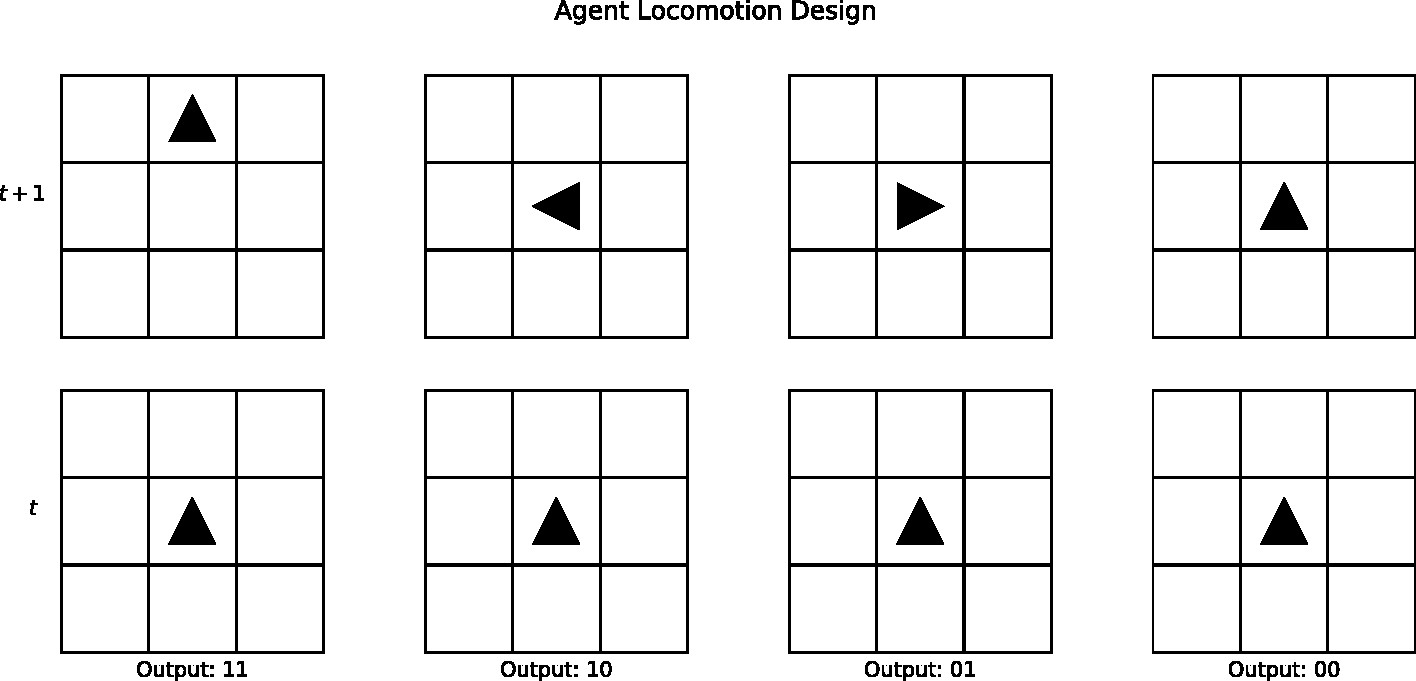
\includegraphics[width=\textwidth]{img/movement_explanatory}
\caption{
Caption TODO
}
\label{fig:movement_explanatory}
\end{center}
\end{figure}


\subsection {Experimental Design}

The hypothesis being tested in this work is that the selective pressures that encourage stigmergy to evolve are those elements of the agent's experience that disrupt the agent's ability to form internal cognitive representations about its environment.
